\documentclass[12pt,a4paper]{article}

% 中文支持
\usepackage{ctex}

% 数学公式
\usepackage{amsmath,amssymb,amsfonts}

% 图形和表格
\usepackage{graphicx}
\usepackage{float}
\usepackage{booktabs}
\usepackage{multirow}
\usepackage{array}

% 代码高亮
\usepackage{listings}
\usepackage{xcolor}

% 页面设置
\usepackage{geometry}
\geometry{left=2.5cm,right=2.5cm,top=2.5cm,bottom=2.5cm}

% 页眉页脚
\usepackage{fancyhdr}
\pagestyle{fancy}
\fancyhf{}
\fancyhead[C]{计算机图形学作业6}
\fancyfoot[C]{\thepage}
\renewcommand{\headrulewidth}{0.4pt}

% 超链接
\usepackage{hyperref}
\hypersetup{
    colorlinks=true,
    linkcolor=blue,
    citecolor=blue,
    urlcolor=blue
}

% 代码样式设置
\lstdefinestyle{cstyle}{
    language=C,
    basicstyle=\ttfamily\small,
    keywordstyle=\color{blue}\bfseries,
    commentstyle=\color{green!60!black}\itshape,
    stringstyle=\color{red},
    numbers=left,
    numberstyle=\tiny\color{gray},
    frame=single,
    framesep=5pt,
    breaklines=true,
    showstringspaces=false,
    tabsize=4,
    captionpos=b,
    xleftmargin=2em,
    framexleftmargin=1.5em
}

\lstdefinestyle{ruststyle}{
    language=C,
    basicstyle=\ttfamily\small,
    keywordstyle=\color{purple}\bfseries,
    commentstyle=\color{green!60!black}\itshape,
    stringstyle=\color{orange},
    numbers=left,
    numberstyle=\tiny\color{gray},
    frame=single,
    framesep=5pt,
    breaklines=true,
    showstringspaces=false,
    tabsize=4,
    captionpos=b,
    xleftmargin=2em,
    framexleftmargin=1.5em,
    morekeywords={fn,let,mut,pub,struct,impl,Self,Vec,usize,f64,bool,true,false}
}

\begin{document}

% ==================== 封面页 ====================
\begin{titlepage}
    \centering
    \vspace*{2cm}
    
    {\Huge\bfseries 计算机图形学\par}
    \vspace{1.5cm}
    
    {\LARGE 作业6\par}
    \vspace{3cm}
    
    \begin{tabular}{rl}
        \textbf{课程名称：} & 计算机图形学 \\[0.5cm]
        \textbf{学\qquad 院：} & \underline{\hspace{5cm}} \\[0.5cm]
        \textbf{专\qquad 业：} & \underline{\hspace{5cm}} \\[0.5cm]
        \textbf{班\qquad 级：} & \underline{\hspace{5cm}} \\[0.5cm]
        \textbf{姓\qquad 名：} & \underline{\hspace{5cm}} \\[0.5cm]
        \textbf{学\qquad 号：} & \underline{\hspace{5cm}} \\[0.5cm]
        \textbf{指导教师：} & \underline{\hspace{5cm}} \\[0.5cm]
    \end{tabular}
    
    \vfill
    
    {\large \today\par}
\end{titlepage}

% ==================== 目录页 ====================
\newpage
\thispagestyle{empty}
\tableofcontents
\newpage
\setcounter{page}{1}

% ==================== 第一题 ====================
\section{三维图形顶点数据结构设计}

\subsection{题目要求}

请根据下面的要求分别设计相应的数据结构用于存储某三维图形的顶点：
\begin{enumerate}
    \item 该三维图形的颜色由顶点的颜色确定。
    \item 在设置不同光照的情况下，该图形的颜色也会发生改变。
    \item 在设置不同纹理的情况下，该图形外表面的粗糙程度也会发生改变。
    \item 在不同光照情况下，可显示出该图形的阴影。
\end{enumerate}

\subsection{设计思路}

为了满足上述四个要求，需要在顶点数据结构中包含以下关键信息：

\begin{itemize}
    \item \textbf{位置坐标}：顶点在三维空间中的位置，是最基本的属性。
    \item \textbf{顶点颜色}：满足要求(1)，通过顶点颜色插值实现图形着色。
    \item \textbf{法向量}：满足要求(2)和(4)，用于光照计算（漫反射、镜面反射）和阴影判断。
    \item \textbf{纹理坐标}：满足要求(3)，用于采样纹理贴图。
    \item \textbf{切线空间向量}：满足要求(3)，用于法线贴图计算，实现表面粗糙度效果。
\end{itemize}

\subsection{数据结构定义}

\subsubsection{基础向量结构}

\begin{lstlisting}[style=ruststyle, caption={基础向量结构定义}]
/// 三维向量结构，用于位置、颜色、法向量等
#[derive(Debug, Clone, Copy)]
pub struct Vec3 {
    pub x: f32,    // X分量
    pub y: f32,    // Y分量
    pub z: f32,    // Z分量
}

/// 二维向量结构，用于纹理坐标
#[derive(Debug, Clone, Copy)]
pub struct Vec2 {
    pub u: f32,    // 纹理U坐标 (水平方向)
    pub v: f32,    // 纹理V坐标 (垂直方向)
}
\end{lstlisting}

\subsubsection{顶点数据结构}

\begin{lstlisting}[style=ruststyle, caption={完整顶点数据结构}]
/// 顶点数据结构
#[derive(Debug, Clone, Copy)]
pub struct Vertex {
    // 基础属性
    pub position: Vec3,      // 顶点位置坐标 (x, y, z)
    
    // 要求(1): 顶点颜色
    pub color: Vec3,         // 顶点颜色 (R, G, B)，范围[0,1]
    
    // 要求(2)(4): 光照和阴影计算
    pub normal: Vec3,        // 顶点法向量，用于光照计算
    
    // 要求(3): 纹理映射
    pub tex_coord: Vec2,     // 纹理坐标 (u, v)
    
    // 要求(3): 切线空间，用于法线贴图实现粗糙度
    pub tangent: Vec3,       // 切线向量
    pub bitangent: Vec3,     // 副切线向量
}
\end{lstlisting}

\subsubsection{辅助数据结构}

为了完整实现光照和材质效果，还需要定义以下辅助结构：

\begin{lstlisting}[style=ruststyle, caption={材质和光源结构}]
/// 材质属性结构
#[derive(Debug, Clone, Copy)]
pub struct Material {
    pub ambient: Vec3,       // 环境光反射系数 (Ka)
    pub diffuse: Vec3,       // 漫反射系数 (Kd)
    pub specular: Vec3,      // 镜面反射系数 (Ks)
    pub shininess: f32,      // 高光指数 (n)
    pub roughness: f32,      // 粗糙度，范围[0,1]
    pub metallic: f32,       // 金属度，范围[0,1]
}

/// 光源类型枚举
#[derive(Debug, Clone, Copy)]
pub enum LightType {
    Point,       // 点光源
    Directional, // 平行光
    Spot,        // 聚光灯
}

/// 光源结构
#[derive(Debug, Clone, Copy)]
pub struct Light {
    pub position: Vec3,      // 光源位置
    pub direction: Vec3,     // 光源方向（用于平行光和聚光灯）
    pub color: Vec3,         // 光源颜色
    pub intensity: f32,      // 光照强度
    pub light_type: LightType, // 光源类型
}

/// 阴影贴图信息
pub struct ShadowMap {
    pub depth_map: Vec<f32>,     // 深度贴图数据
    pub width: usize,            // 贴图宽度
    pub height: usize,           // 贴图高度
    pub light_matrix: [f32; 16], // 光源空间变换矩阵
}
\end{lstlisting}

\subsection{各字段详细说明}

\begin{table}[H]
\centering
\caption{顶点数据结构字段说明}
\begin{tabular}{|c|c|c|p{6cm}|}
\hline
\textbf{字段} & \textbf{类型} & \textbf{对应要求} & \textbf{功能说明} \\
\hline
position & Vec3 & 基础 & 存储顶点在世界坐标系中的位置$(x,y,z)$ \\
\hline
color & Vec3 & 要求(1) & 存储顶点RGB颜色，通过重心坐标插值确定片元颜色 \\
\hline
normal & Vec3 & 要求(2)(4) & 存储顶点法向量，用于计算光照强度和阴影 \\
\hline
texCoord & Vec2 & 要求(3) & 存储纹理坐标$(u,v)$，用于采样纹理贴图 \\
\hline
tangent & Vec3 & 要求(3) & 切线向量，与normal、bitangent构成TBN矩阵 \\
\hline
bitangent & Vec3 & 要求(3) & 副切线向量，用于法线贴图的切线空间变换 \\
\hline
\end{tabular}
\end{table}

\subsection{光照计算原理}

\subsubsection{Phong光照模型}

满足要求(2)，使用Phong光照模型计算顶点颜色：

\begin{equation}
I = I_a \cdot K_a + I_d \cdot K_d \cdot (\vec{N} \cdot \vec{L}) + I_s \cdot K_s \cdot (\vec{R} \cdot \vec{V})^n
\end{equation}

其中：
\begin{itemize}
    \item $I_a, I_d, I_s$：环境光、漫反射光、镜面反射光强度
    \item $K_a, K_d, K_s$：材质的环境光、漫反射、镜面反射系数
    \item $\vec{N}$：顶点法向量（来自normal字段）
    \item $\vec{L}$：光源方向向量
    \item $\vec{R}$：反射光方向向量
    \item $\vec{V}$：视线方向向量
    \item $n$：高光指数
\end{itemize}

\subsubsection{阴影映射算法}

满足要求(4)，使用Shadow Mapping算法实现阴影：

\begin{enumerate}
    \item 从光源视角渲染场景，生成深度贴图（Shadow Map）
    \item 渲染场景时，将每个片元变换到光源空间
    \item 比较片元深度与深度贴图中的值，判断是否在阴影中
\end{enumerate}

\subsubsection{法线贴图与粗糙度}

满足要求(3)，通过TBN矩阵实现法线贴图：

\begin{equation}
TBN = \begin{bmatrix}
T_x & B_x & N_x \\
T_y & B_y & N_y \\
T_z & B_z & N_z
\end{bmatrix}
\end{equation}

其中$\vec{T}$（tangent）、$\vec{B}$（bitangent）、$\vec{N}$（normal）构成切线空间的正交基。通过法线贴图可以在不增加几何复杂度的情况下模拟表面粗糙度变化。


% ==================== 第二题 ====================
\newpage
\section{三阶B样条曲面设计与实现}

\subsection{题目要求}

编写程序，设计一个三阶的B样条曲面，在给定控制点的情况下，计算出B样条曲面上的点（设$u$，$v$方向的曲面精度可通过参数设置），然后将这些点保存到数组中。如果该B样条曲面以三角面为基本图元进行存储，计算出三角形顶点的索引，并保存到数组中。采用Rust语言。

\subsection{B样条曲面理论基础}

\subsubsection{B样条基函数}

B样条基函数采用Cox-de Boor递推公式定义。设节点向量为$\{t_0, t_1, \ldots, t_m\}$，则$p$次B样条基函数定义为：

\textbf{零次基函数}（$p=0$）：
\begin{equation}
N_{i,0}(t) = \begin{cases}
1 & \text{若 } t_i \leq t < t_{i+1} \\
0 & \text{其他}
\end{cases}
\end{equation}

\textbf{递推公式}（$p \geq 1$）：
\begin{equation}
N_{i,p}(t) = \frac{t - t_i}{t_{i+p} - t_i} N_{i,p-1}(t) + \frac{t_{i+p+1} - t}{t_{i+p+1} - t_{i+1}} N_{i+1,p-1}(t)
\end{equation}

其中，当分母为零时，约定该项为零。

\subsubsection{B样条曲面定义}

给定$m \times n$个控制点$\mathbf{P}_{i,j}$（$i=0,1,\ldots,m-1$；$j=0,1,\ldots,n-1$），$p$次$\times$ $q$次B样条曲面定义为：

\begin{equation}
\mathbf{S}(u,v) = \sum_{i=0}^{m-1} \sum_{j=0}^{n-1} N_{i,p}(u) \cdot N_{j,q}(v) \cdot \mathbf{P}_{i,j}
\end{equation}

对于三阶B样条曲面，$p = q = 3$（即3次B样条）。

\subsubsection{节点向量}

对于$n$个控制点和$p$次B样条，节点向量包含$n+p+1$个节点。本实现采用均匀开放节点向量：

\begin{equation}
t_i = \begin{cases}
0 & i \leq p \\
\frac{i-p}{n-p} & p < i < n \\
1 & i \geq n
\end{cases}
\end{equation}

\subsection{三角形网格生成}

\subsubsection{曲面离散化}

将参数域$[0,1] \times [0,1]$按照给定精度离散化：
\begin{itemize}
    \item $u$方向细分为$u_{res}$段，共$u_{res}+1$个采样点
    \item $v$方向细分为$v_{res}$段，共$v_{res}+1$个采样点
    \item 总顶点数：$(u_{res}+1) \times (v_{res}+1)$
\end{itemize}

\subsubsection{三角形索引生成}

每个网格单元划分为两个三角形。对于网格点$(i,j)$，其在顶点数组中的索引为：
\begin{equation}
idx(i,j) = i \times (v_{res}+1) + j
\end{equation}

两个三角形的顶点索引为：
\begin{itemize}
    \item \textbf{三角形1}：$(idx(i,j), \; idx(i,j+1), \; idx(i+1,j+1))$
    \item \textbf{三角形2}：$(idx(i,j), \; idx(i+1,j+1), \; idx(i+1,j))$
\end{itemize}

总三角形数量：$2 \times u_{res} \times v_{res}$

\begin{figure}[H]
\centering
\begin{verbatim}
    (i+1,j) -------- (i+1,j+1)
       |  \    T2    |
       |    \        |
       |  T1  \      |
       |        \    |
    (i,j) -------- (i,j+1)
\end{verbatim}
\caption{网格单元三角形划分示意图}
\end{figure}

\subsection{Rust代码实现}

\subsubsection{数据结构定义}

\begin{lstlisting}[style=ruststyle, caption={三维点结构}]
/// 三维点结构
#[derive(Debug, Clone, Copy)]
pub struct Point3 {
    pub x: f64,
    pub y: f64,
    pub z: f64,
}

impl Point3 {
    /// 创建新的三维点
    pub fn new(x: f64, y: f64, z: f64) -> Self {
        Self { x, y, z }
    }

    /// 创建零点
    pub fn zero() -> Self {
        Self { x: 0.0, y: 0.0, z: 0.0 }
    }
}

/// 实现加法运算
impl std::ops::Add for Point3 {
    type Output = Self;
    fn add(self, other: Self) -> Self {
        Self {
            x: self.x + other.x,
            y: self.y + other.y,
            z: self.z + other.z,
        }
    }
}

/// 实现标量乘法
impl std::ops::Mul<f64> for Point3 {
    type Output = Self;
    fn mul(self, scalar: f64) -> Self {
        Self {
            x: self.x * scalar,
            y: self.y * scalar,
            z: self.z * scalar,
        }
    }
}
\end{lstlisting}

\subsubsection{B样条曲面结构}

\begin{lstlisting}[style=ruststyle, caption={B样条曲面结构}]
/// B样条曲面结构
pub struct BSplineSurface {
    control_points: Vec<Vec<Point3>>,  // m x n 控制点网格
    knots_u: Vec<f64>,                  // u方向节点向量
    knots_v: Vec<f64>,                  // v方向节点向量
    degree: usize,                       // 曲线次数
}

impl BSplineSurface {
    /// 创建三阶B样条曲面
    /// 参数: control_points - m x n 控制点网格
    pub fn new(control_points: Vec<Vec<Point3>>) -> Self {
        let m = control_points.len();
        let n = control_points[0].len();
        let degree = 3; // 三阶B样条，次数为3

        // 生成均匀开放节点向量
        let knots_u = Self::generate_uniform_knots(m, degree);
        let knots_v = Self::generate_uniform_knots(n, degree);

        Self {
            control_points,
            knots_u,
            knots_v,
            degree,
        }
    }

    /// 生成均匀开放节点向量
    fn generate_uniform_knots(n: usize, degree: usize) -> Vec<f64> {
        let num_knots = n + degree + 1;
        let mut knots = Vec::with_capacity(num_knots);
        
        for i in 0..num_knots {
            if i <= degree {
                knots.push(0.0);  // 前degree+1个节点为0
            } else if i >= num_knots - degree - 1 {
                knots.push(1.0);  // 后degree+1个节点为1
            } else {
                // 中间节点均匀分布
                let val = (i - degree) as f64 
                        / (num_knots - 2 * degree - 1) as f64;
                knots.push(val);
            }
        }
        knots
    }
}
\end{lstlisting}

\subsubsection{基函数计算}

\begin{lstlisting}[style=ruststyle, caption={Cox-de Boor递推算法}]
impl BSplineSurface {
    /// Cox-de Boor递推公式计算B样条基函数
    /// 参数: i - 基函数索引, p - 次数, t - 参数值, knots - 节点向量
    fn basis_function(&self, i: usize, p: usize, t: f64, 
                      knots: &[f64]) -> f64 {
        // 零次基函数
        if p == 0 {
            if knots[i] <= t && t < knots[i + 1] {
                return 1.0;
            }
            // 处理 t = 1.0 的边界情况
            if (t - 1.0).abs() < 1e-10 
               && (knots[i + 1] - 1.0).abs() < 1e-10 {
                return 1.0;
            }
            return 0.0;
        }

        // 递推计算
        let mut result = 0.0;

        // 第一项
        let denom1 = knots[i + p] - knots[i];
        if denom1.abs() > 1e-10 {
            result += (t - knots[i]) / denom1 
                    * self.basis_function(i, p - 1, t, knots);
        }

        // 第二项
        let denom2 = knots[i + p + 1] - knots[i + 1];
        if denom2.abs() > 1e-10 {
            result += (knots[i + p + 1] - t) / denom2 
                    * self.basis_function(i + 1, p - 1, t, knots);
        }

        result
    }

    /// 计算曲面上一点 S(u,v)
    pub fn evaluate(&self, u: f64, v: f64) -> Point3 {
        let m = self.control_points.len();
        let n = self.control_points[0].len();
        let mut point = Point3::zero();

        // 双重求和
        for i in 0..m {
            let basis_u = self.basis_function(i, self.degree, 
                                              u, &self.knots_u);
            for j in 0..n {
                let basis_v = self.basis_function(j, self.degree, 
                                                  v, &self.knots_v);
                let weight = basis_u * basis_v;
                point = point + self.control_points[i][j] * weight;
            }
        }

        point
    }
}
\end{lstlisting}

\subsubsection{网格生成}

\begin{lstlisting}[style=ruststyle, caption={曲面网格生成}]
impl BSplineSurface {
    /// 生成曲面点和三角形索引
    /// 参数: u_resolution - u方向细分数
    ///       v_resolution - v方向细分数
    /// 返回: (顶点数组, 三角形索引数组)
    pub fn generate_mesh(&self, u_resolution: usize, 
                         v_resolution: usize) 
        -> (Vec<Point3>, Vec<[usize; 3]>) 
    {
        let mut vertices = Vec::new();
        let mut indices = Vec::new();

        // 生成曲面上的点
        for i in 0..=u_resolution {
            let u = i as f64 / u_resolution as f64;
            for j in 0..=v_resolution {
                let v = j as f64 / v_resolution as f64;
                vertices.push(self.evaluate(u, v));
            }
        }

        // 生成三角形索引
        let cols = v_resolution + 1;
        for i in 0..u_resolution {
            for j in 0..v_resolution {
                let idx = i * cols + j;
                
                // 三角形1: 左下-右下-右上
                indices.push([idx, idx + 1, idx + cols + 1]);
                
                // 三角形2: 左下-右上-左上
                indices.push([idx, idx + cols + 1, idx + cols]);
            }
        }

        (vertices, indices)
    }
}
\end{lstlisting}

\subsection{程序运行结果}

使用$4 \times 4$控制点网格，$u$和$v$方向各细分10段，程序运行结果如图\ref{fig:bspline_result1}和图\ref{fig:bspline_result2}所示。

\begin{figure}[H]
\centering
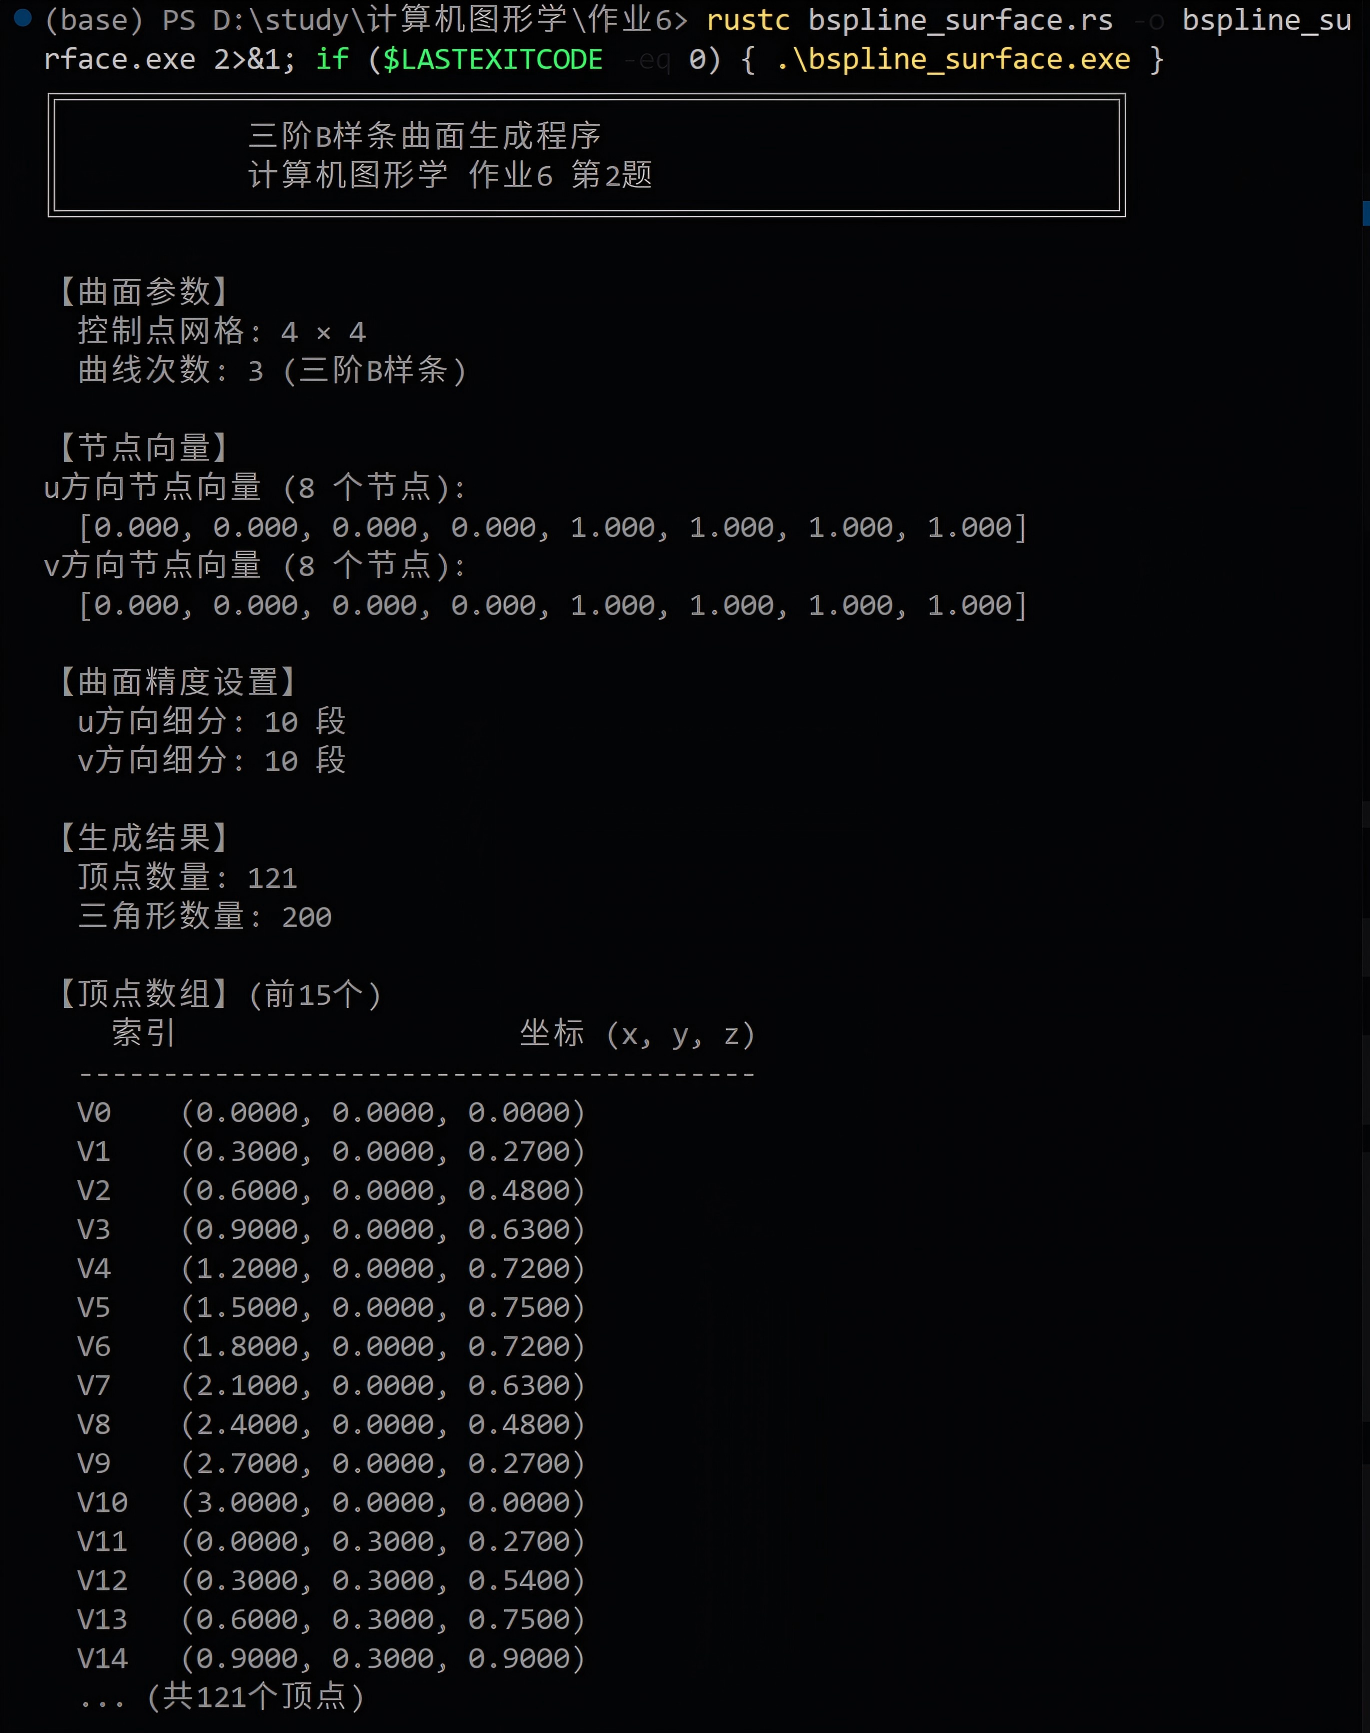
\includegraphics[width=0.9\textwidth]{1.png}
\caption{三阶B样条曲面程序运行结果（一）}
\label{fig:bspline_result1}
\end{figure}

\begin{figure}[H]
\centering
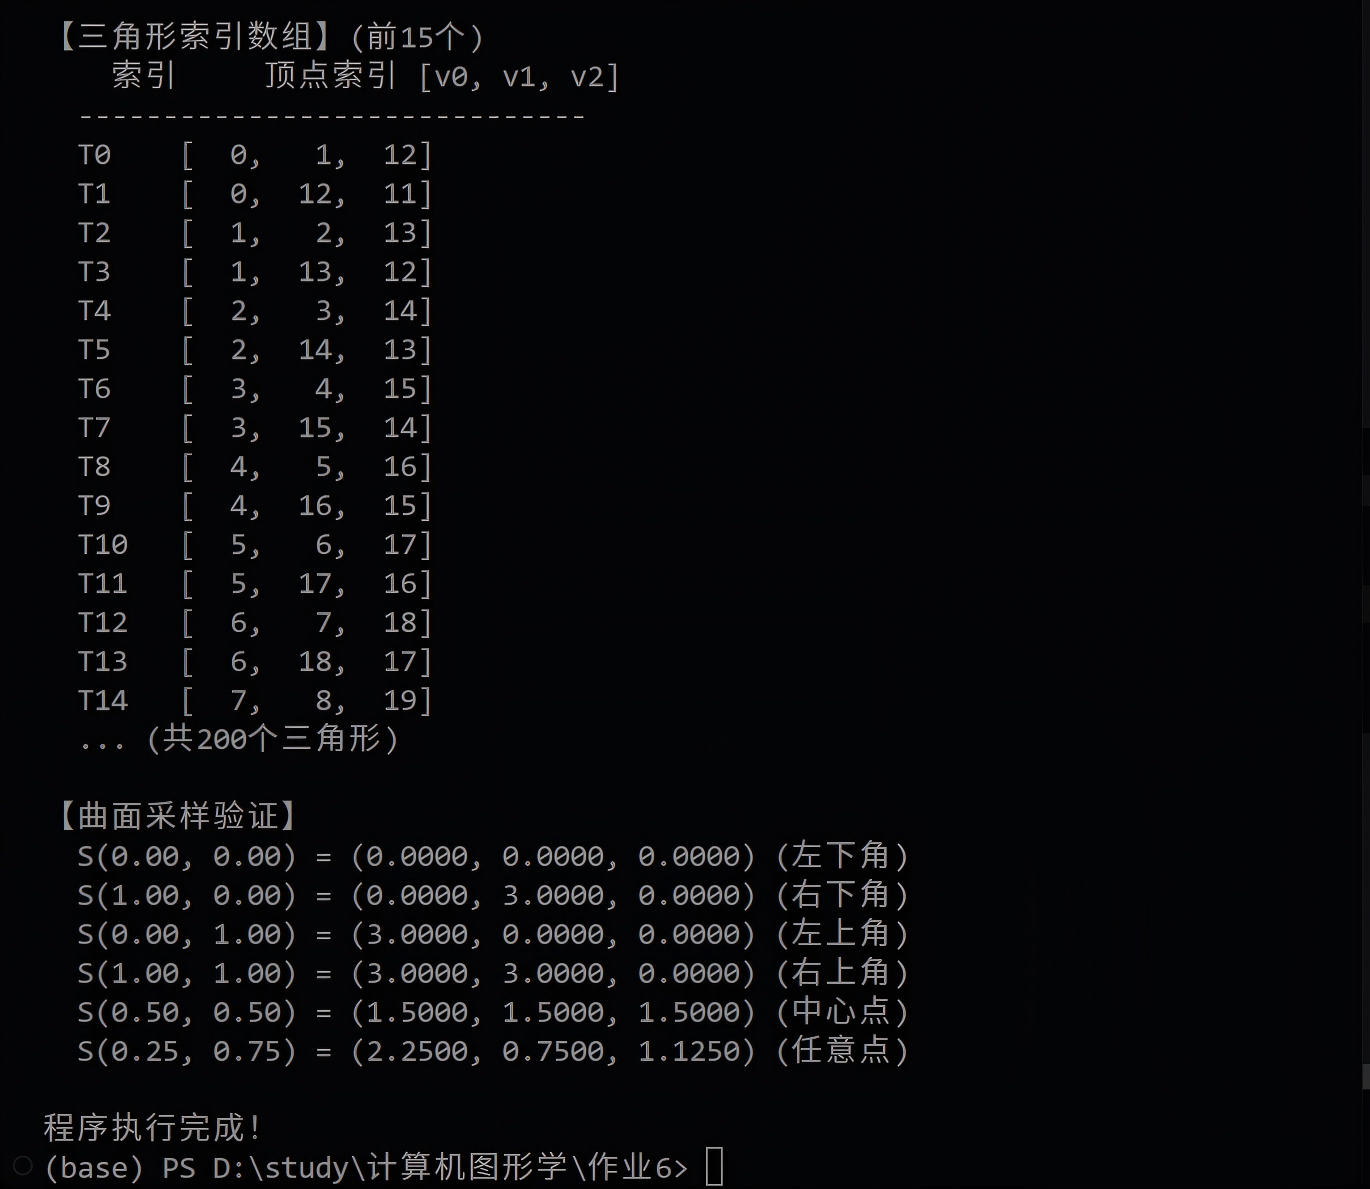
\includegraphics[width=0.9\textwidth]{2.png}
\caption{三阶B样条曲面程序运行结果（二）}
\label{fig:bspline_result2}
\end{figure}

程序输出的主要内容包括：
\begin{itemize}
    \item 曲面参数信息：控制点网格大小、曲线次数
    \item 节点向量：u方向和v方向的均匀开放节点向量
    \item 生成结果统计：顶点数量121个，三角形数量200个
    \item 顶点数组：存储曲面上离散点的三维坐标
    \item 三角形索引数组：存储三角形顶点的索引关系
    \item 曲面采样验证：验证曲面角点和中心点的坐标值
\end{itemize}


% ==================== 第三题 ====================
\newpage
\section{正方体纹理坐标设计}

\subsection{题目要求}

一张图片上有8个不同的数字，每个数字的宽度和长度均相同。现希望将其前6个数字作为纹理贴到一个正方体的六个面上，使每个面上分别显示出不同的数字，请问如何设计该正方形每个顶点的纹理坐标。

\subsection{问题分析}

\subsubsection{纹理图片布局}

假设8个数字在图片中水平排列（$8 \times 1$布局），则：
\begin{itemize}
    \item 图片总宽度归一化为1.0
    \item 每个数字占据宽度：$\frac{1}{8} = 0.125$
    \item 图片高度归一化为1.0
    \item 第$n$个数字（$n=0,1,\ldots,7$）的纹理坐标范围：
    \begin{equation}
    u \in \left[\frac{n}{8}, \frac{n+1}{8}\right], \quad v \in [0, 1]
    \end{equation}
\end{itemize}

\begin{figure}[H]
\centering
\begin{verbatim}
+-----+-----+-----+-----+-----+-----+-----+-----+
|  0  |  1  |  2  |  3  |  4  |  5  |  6  |  7  |
+-----+-----+-----+-----+-----+-----+-----+-----+
0   0.125 0.25 0.375 0.5  0.625 0.75 0.875  1.0  (u坐标)
\end{verbatim}
\caption{纹理图片布局示意图（8个数字水平排列）}
\end{figure}

\subsubsection{正方体顶点定义}

设正方体边长为2，中心位于原点，则8个顶点坐标为：

\begin{table}[H]
\centering
\caption{正方体顶点坐标}
\begin{tabular}{|c|c|c|c|}
\hline
\textbf{顶点} & \textbf{X} & \textbf{Y} & \textbf{Z} \\
\hline
$V_0$ & $-1$ & $-1$ & $-1$ \\
$V_1$ & $+1$ & $-1$ & $-1$ \\
$V_2$ & $+1$ & $+1$ & $-1$ \\
$V_3$ & $-1$ & $+1$ & $-1$ \\
$V_4$ & $-1$ & $-1$ & $+1$ \\
$V_5$ & $+1$ & $-1$ & $+1$ \\
$V_6$ & $+1$ & $+1$ & $+1$ \\
$V_7$ & $-1$ & $+1$ & $+1$ \\
\hline
\end{tabular}
\end{table}

\begin{figure}[H]
\centering
\begin{verbatim}
        V7 -------- V6
       /|         /|
      / |        / |
     V3 -------- V2|
     |  |       |  |
     |  V4 -----|-- V5
     | /        | /
     |/         |/
     V0 -------- V1
     
     Y
     |  Z
     | /
     |/_____ X
\end{verbatim}
\caption{正方体顶点编号示意图}
\end{figure}

\subsection{各面纹理坐标设计}

\subsubsection{纹理坐标映射原则}

对于每个面，需要将四个顶点映射到对应数字的纹理区域。设第$n$个数字的纹理坐标边界为：
\begin{align}
u_{min} &= \frac{n}{8} \\
u_{max} &= \frac{n+1}{8} \\
v_{min} &= 0 \\
v_{max} &= 1
\end{align}

四个角的纹理坐标为：
\begin{itemize}
    \item 左下角：$(u_{min}, v_{min})$
    \item 右下角：$(u_{max}, v_{min})$
    \item 右上角：$(u_{max}, v_{max})$
    \item 左上角：$(u_{min}, v_{max})$
\end{itemize}

\subsubsection{六个面的详细设计}

\paragraph{面1：前面（+Z方向）- 数字0}

\begin{itemize}
    \item 顶点顺序：$V_4 \to V_5 \to V_6 \to V_7$（逆时针）
    \item 数字编号：0
    \item 纹理范围：$u \in [0, 0.125]$, $v \in [0, 1]$
\end{itemize}

\begin{table}[H]
\centering
\begin{tabular}{|c|c|c|c|}
\hline
\textbf{顶点} & \textbf{位置坐标} & \textbf{纹理坐标} & \textbf{位置} \\
\hline
$V_4$ & $(-1, -1, +1)$ & $(0.000, 0)$ & 左下 \\
$V_5$ & $(+1, -1, +1)$ & $(0.125, 0)$ & 右下 \\
$V_6$ & $(+1, +1, +1)$ & $(0.125, 1)$ & 右上 \\
$V_7$ & $(-1, +1, +1)$ & $(0.000, 1)$ & 左上 \\
\hline
\end{tabular}
\end{table}

\paragraph{面2：后面（-Z方向）- 数字1}

\begin{itemize}
    \item 顶点顺序：$V_1 \to V_0 \to V_3 \to V_2$（从后面看逆时针）
    \item 数字编号：1
    \item 纹理范围：$u \in [0.125, 0.25]$, $v \in [0, 1]$
\end{itemize}

\begin{table}[H]
\centering
\begin{tabular}{|c|c|c|c|}
\hline
\textbf{顶点} & \textbf{位置坐标} & \textbf{纹理坐标} & \textbf{位置} \\
\hline
$V_1$ & $(+1, -1, -1)$ & $(0.125, 0)$ & 左下 \\
$V_0$ & $(-1, -1, -1)$ & $(0.250, 0)$ & 右下 \\
$V_3$ & $(-1, +1, -1)$ & $(0.250, 1)$ & 右上 \\
$V_2$ & $(+1, +1, -1)$ & $(0.125, 1)$ & 左上 \\
\hline
\end{tabular}
\end{table}

\paragraph{面3：左面（-X方向）- 数字2}

\begin{itemize}
    \item 顶点顺序：$V_0 \to V_4 \to V_7 \to V_3$（从左面看逆时针）
    \item 数字编号：2
    \item 纹理范围：$u \in [0.25, 0.375]$, $v \in [0, 1]$
\end{itemize}

\begin{table}[H]
\centering
\begin{tabular}{|c|c|c|c|}
\hline
\textbf{顶点} & \textbf{位置坐标} & \textbf{纹理坐标} & \textbf{位置} \\
\hline
$V_0$ & $(-1, -1, -1)$ & $(0.250, 0)$ & 左下 \\
$V_4$ & $(-1, -1, +1)$ & $(0.375, 0)$ & 右下 \\
$V_7$ & $(-1, +1, +1)$ & $(0.375, 1)$ & 右上 \\
$V_3$ & $(-1, +1, -1)$ & $(0.250, 1)$ & 左上 \\
\hline
\end{tabular}
\end{table}

\paragraph{面4：右面（+X方向）- 数字3}

\begin{itemize}
    \item 顶点顺序：$V_5 \to V_1 \to V_2 \to V_6$（从右面看逆时针）
    \item 数字编号：3
    \item 纹理范围：$u \in [0.375, 0.5]$, $v \in [0, 1]$
\end{itemize}

\begin{table}[H]
\centering
\begin{tabular}{|c|c|c|c|}
\hline
\textbf{顶点} & \textbf{位置坐标} & \textbf{纹理坐标} & \textbf{位置} \\
\hline
$V_5$ & $(+1, -1, +1)$ & $(0.375, 0)$ & 左下 \\
$V_1$ & $(+1, -1, -1)$ & $(0.500, 0)$ & 右下 \\
$V_2$ & $(+1, +1, -1)$ & $(0.500, 1)$ & 右上 \\
$V_6$ & $(+1, +1, +1)$ & $(0.375, 1)$ & 左上 \\
\hline
\end{tabular}
\end{table}

\paragraph{面5：上面（+Y方向）- 数字4}

\begin{itemize}
    \item 顶点顺序：$V_3 \to V_7 \to V_6 \to V_2$（从上面看逆时针）
    \item 数字编号：4
    \item 纹理范围：$u \in [0.5, 0.625]$, $v \in [0, 1]$
\end{itemize}

\begin{table}[H]
\centering
\begin{tabular}{|c|c|c|c|}
\hline
\textbf{顶点} & \textbf{位置坐标} & \textbf{纹理坐标} & \textbf{位置} \\
\hline
$V_3$ & $(-1, +1, -1)$ & $(0.500, 0)$ & 左下 \\
$V_7$ & $(-1, +1, +1)$ & $(0.625, 0)$ & 右下 \\
$V_6$ & $(+1, +1, +1)$ & $(0.625, 1)$ & 右上 \\
$V_2$ & $(+1, +1, -1)$ & $(0.500, 1)$ & 左上 \\
\hline
\end{tabular}
\end{table}

\paragraph{面6：下面（-Y方向）- 数字5}

\begin{itemize}
    \item 顶点顺序：$V_4 \to V_0 \to V_1 \to V_5$（从下面看逆时针）
    \item 数字编号：5
    \item 纹理范围：$u \in [0.625, 0.75]$, $v \in [0, 1]$
\end{itemize}

\begin{table}[H]
\centering
\begin{tabular}{|c|c|c|c|}
\hline
\textbf{顶点} & \textbf{位置坐标} & \textbf{纹理坐标} & \textbf{位置} \\
\hline
$V_4$ & $(-1, -1, +1)$ & $(0.625, 0)$ & 左下 \\
$V_0$ & $(-1, -1, -1)$ & $(0.750, 0)$ & 右下 \\
$V_1$ & $(+1, -1, -1)$ & $(0.750, 1)$ & 右上 \\
$V_5$ & $(+1, -1, +1)$ & $(0.625, 1)$ & 左上 \\
\hline
\end{tabular}
\end{table}

\subsection{纹理坐标汇总表}

\begin{table}[H]
\centering
\caption{正方体六个面纹理坐标汇总}
\begin{tabular}{|c|c|c|c|c|c|c|}
\hline
\textbf{面} & \textbf{方向} & \textbf{数字} & \textbf{左下} & \textbf{右下} & \textbf{右上} & \textbf{左上} \\
\hline
前面 & +Z & 0 & (0.000, 0) & (0.125, 0) & (0.125, 1) & (0.000, 1) \\
\hline
后面 & -Z & 1 & (0.125, 0) & (0.250, 0) & (0.250, 1) & (0.125, 1) \\
\hline
左面 & -X & 2 & (0.250, 0) & (0.375, 0) & (0.375, 1) & (0.250, 1) \\
\hline
右面 & +X & 3 & (0.375, 0) & (0.500, 0) & (0.500, 1) & (0.375, 1) \\
\hline
上面 & +Y & 4 & (0.500, 0) & (0.625, 0) & (0.625, 1) & (0.500, 1) \\
\hline
下面 & -Y & 5 & (0.625, 0) & (0.750, 0) & (0.750, 1) & (0.625, 1) \\
\hline
\end{tabular}
\end{table}

\subsection{代码实现示例}

\begin{lstlisting}[style=ruststyle, caption={正方体纹理坐标定义}]
/// 二维向量，用于纹理坐标
#[derive(Debug, Clone, Copy)]
pub struct Vec2 {
    pub u: f32,
    pub v: f32,
}

/// 三维向量，用于位置坐标
#[derive(Debug, Clone, Copy)]
pub struct Vec3 {
    pub x: f32,
    pub y: f32,
    pub z: f32,
}

/// 正方体顶点（含纹理坐标）
#[derive(Debug, Clone, Copy)]
pub struct CubeVertex {
    pub position: Vec3,
    pub tex_coord: Vec2,
}

/// 生成正方体顶点数据（每个面4个顶点，共24个）
/// 因为同一顶点在不同面有不同纹理坐标
pub fn create_cube_vertices() -> [CubeVertex; 24] {
    [
        // 前面 (+Z) - 数字0
        CubeVertex { position: Vec3 { x: -1.0, y: -1.0, z: 1.0 }, 
                     tex_coord: Vec2 { u: 0.000, v: 0.0 } },  // V4 左下
        CubeVertex { position: Vec3 { x: 1.0, y: -1.0, z: 1.0 }, 
                     tex_coord: Vec2 { u: 0.125, v: 0.0 } },  // V5 右下
        CubeVertex { position: Vec3 { x: 1.0, y: 1.0, z: 1.0 }, 
                     tex_coord: Vec2 { u: 0.125, v: 1.0 } },  // V6 右上
        CubeVertex { position: Vec3 { x: -1.0, y: 1.0, z: 1.0 }, 
                     tex_coord: Vec2 { u: 0.000, v: 1.0 } },  // V7 左上
        
        // 后面 (-Z) - 数字1
        CubeVertex { position: Vec3 { x: 1.0, y: -1.0, z: -1.0 }, 
                     tex_coord: Vec2 { u: 0.125, v: 0.0 } },  // V1 左下
        CubeVertex { position: Vec3 { x: -1.0, y: -1.0, z: -1.0 }, 
                     tex_coord: Vec2 { u: 0.250, v: 0.0 } },  // V0 右下
        CubeVertex { position: Vec3 { x: -1.0, y: 1.0, z: -1.0 }, 
                     tex_coord: Vec2 { u: 0.250, v: 1.0 } },  // V3 右上
        CubeVertex { position: Vec3 { x: 1.0, y: 1.0, z: -1.0 }, 
                     tex_coord: Vec2 { u: 0.125, v: 1.0 } },  // V2 左上
        
        // 左面 (-X) - 数字2
        CubeVertex { position: Vec3 { x: -1.0, y: -1.0, z: -1.0 }, 
                     tex_coord: Vec2 { u: 0.250, v: 0.0 } },  // V0 左下
        CubeVertex { position: Vec3 { x: -1.0, y: -1.0, z: 1.0 }, 
                     tex_coord: Vec2 { u: 0.375, v: 0.0 } },  // V4 右下
        CubeVertex { position: Vec3 { x: -1.0, y: 1.0, z: 1.0 }, 
                     tex_coord: Vec2 { u: 0.375, v: 1.0 } },  // V7 右上
        CubeVertex { position: Vec3 { x: -1.0, y: 1.0, z: -1.0 }, 
                     tex_coord: Vec2 { u: 0.250, v: 1.0 } },  // V3 左上
        
        // 右面 (+X) - 数字3
        CubeVertex { position: Vec3 { x: 1.0, y: -1.0, z: 1.0 }, 
                     tex_coord: Vec2 { u: 0.375, v: 0.0 } },  // V5 左下
        CubeVertex { position: Vec3 { x: 1.0, y: -1.0, z: -1.0 }, 
                     tex_coord: Vec2 { u: 0.500, v: 0.0 } },  // V1 右下
        CubeVertex { position: Vec3 { x: 1.0, y: 1.0, z: -1.0 }, 
                     tex_coord: Vec2 { u: 0.500, v: 1.0 } },  // V2 右上
        CubeVertex { position: Vec3 { x: 1.0, y: 1.0, z: 1.0 }, 
                     tex_coord: Vec2 { u: 0.375, v: 1.0 } },  // V6 左上
        
        // 上面 (+Y) - 数字4
        CubeVertex { position: Vec3 { x: -1.0, y: 1.0, z: -1.0 }, 
                     tex_coord: Vec2 { u: 0.500, v: 0.0 } },  // V3 左下
        CubeVertex { position: Vec3 { x: -1.0, y: 1.0, z: 1.0 }, 
                     tex_coord: Vec2 { u: 0.625, v: 0.0 } },  // V7 右下
        CubeVertex { position: Vec3 { x: 1.0, y: 1.0, z: 1.0 }, 
                     tex_coord: Vec2 { u: 0.625, v: 1.0 } },  // V6 右上
        CubeVertex { position: Vec3 { x: 1.0, y: 1.0, z: -1.0 }, 
                     tex_coord: Vec2 { u: 0.500, v: 1.0 } },  // V2 左上
        
        // 下面 (-Y) - 数字5
        CubeVertex { position: Vec3 { x: -1.0, y: -1.0, z: 1.0 }, 
                     tex_coord: Vec2 { u: 0.625, v: 0.0 } },  // V4 左下
        CubeVertex { position: Vec3 { x: -1.0, y: -1.0, z: -1.0 }, 
                     tex_coord: Vec2 { u: 0.750, v: 0.0 } },  // V0 右下
        CubeVertex { position: Vec3 { x: 1.0, y: -1.0, z: -1.0 }, 
                     tex_coord: Vec2 { u: 0.750, v: 1.0 } },  // V1 右上
        CubeVertex { position: Vec3 { x: 1.0, y: -1.0, z: 1.0 }, 
                     tex_coord: Vec2 { u: 0.625, v: 1.0 } },  // V5 左上
    ]
}

/// 生成三角形索引（每个面2个三角形，共36个索引）
pub fn create_cube_indices() -> [u32; 36] {
    [
        0, 1, 2,  0, 2, 3,      // 前面
        4, 5, 6,  4, 6, 7,      // 后面
        8, 9, 10, 8, 10, 11,    // 左面
        12, 13, 14, 12, 14, 15, // 右面
        16, 17, 18, 16, 18, 19, // 上面
        20, 21, 22, 20, 22, 23, // 下面
    ]
}
\end{lstlisting}

\subsection{注意事项}

\begin{enumerate}
    \item \textbf{顶点重复}：由于同一个几何顶点在不同面上需要不同的纹理坐标，因此正方体需要24个顶点（而非8个）来存储完整的纹理映射信息。
    
    \item \textbf{纹理方向}：需要确保纹理在每个面上的方向正确，避免数字显示颠倒或镜像。
    
    \item \textbf{纹理过滤}：在纹理边界处可能出现采样问题，建议在数字之间留出少量边距，或使用GL\_CLAMP\_TO\_EDGE等纹理包裹模式。
    
    \item \textbf{面的朝向}：顶点顺序决定了面的法向量方向，需要保持一致的绑定顺序（如逆时针为正面）。
\end{enumerate}

\end{document}
